\appendix
\renewcommand{\theequation}{A.\arabic{section}.\arabic{equation}}
\setcounter{equation}{0}

\section{物理数学}

\subsection{$L^p$-norm}

$\mathbb{R}^n$または
$\mathbb{C}^n$上の
$n$次元vector $v$に対し、
実数$1\le p < \infty$の範囲で
$L^p$-normを
\begin{align}
    ||v||_p
:=
    \left(
        \sum_{i=1}^n
        |v_i|^p
    \right)^{ \dfrac{1}{p} }
\end{align}
と定義する。
$p\to\infty$の極限を
$L^\infty$-normないし最大値normと言い、
\begin{align}
    ||v||_\infty
=
    \max_i
    |v_i|
\end{align}
に一致する。
特に$n \to \infty$(つまり無限数列)の場合、
上の$p$-normを有限にするようなvectorの集合を$l^p$と呼ぶ。

測度空間についても
和を積分に置き換えることにより同様のnormが定義でき、
これを有限にする可測関数の集合を
$L^p$空間と呼ぶ。

\subsection{複素関数論}

\subsubsection{Taylor series expansion(テイラー級数展開)}

実関数$f(x)$が点$a$で無限回微分可能であるとする。
\begin{subequations}
\begin{align}
    f(x)
    =
    \sum_{n=0}^{\infty}
    \dfrac{ f^{n}(a) }{n!}
    (x-a)^n
\\
    f^{n}(a) := \dfrac{d^nf}{dx^n}\bigg|_{x=a}
\end{align}
\end{subequations}
を$f(x)$の$a$周りでのTaylor展開という。
特に
$a=0$とした場合のTaylor展開を
Maclaurin series expansion(マクローリン展開)とも言う。
Taylor展開が収束し、
かつ元の関数$f(x)$に一致するとき
$f(x)$はTaylor展開可能であるという。
例えば$\exp(-1/x^2)$は$x=0$で無限回微分可能であり
そのTaylor展開も収束するが、
恒等的に$0$になって$\exp(-1/x^2)$に一致しない。
従って$\exp(-1/x^2)$は$x=0$まわりでTaylor展開可能ではない
(このことは、$\exp(-1/x^2)$を複素関数と見たとき
$x=0$が真性特異点となっている事実を反映している)。

複素関数$f(z)$が領域$D$で正則であるとする。
点$a$を中心とする領域$D$内の任意の円$C$に対し、
$f(z)$は$C$の内部で
\begin{subequations}
\begin{align}
    f(z)
    &=
    \sum_{n=0}^{\infty}
    \dfrac{f^{(n)}(a)}{n!}
    (z-a)^n
\\
    f^{(n)}(a)
    &=
    \dfrac{n!}{2 \pi i}
    \oint_C dz_0\dfrac{f(z_0)}{(z_0 - a)^{n+1}}
\label{Cauchy's integral formula}
\end{align}
\end{subequations}
とべき級数展開できる。
なお
(\ref{Cauchy's integral formula})
は$f(a)$の$n$階の導関数を与え、
特に$n=0$の場合を指して
Cauchy's integral formula(コーシーの積分公式)
と呼ぶことがある。

Taylor展開可能な実関数または複素関数を解析関数(analytic function)という。
$f(z)$が複素関数の意味で$z$により微分できるとき
正則関数(holomorphic function)と言うのであったが、
複素関数は領域$D$で正則であれば無限階微分可能であり、
しかもその導関数も$D$で正則なので、
複素関数に対して解析関数と正則関数はほとんど区別しない。

\subsubsection{Laurent series expansion(ローラン級数展開)}

\begin{wrapfigure}[7]{r}[5pt]{107pt}
  \centering
  

\tikzset{every picture/.style={line width=0.75pt}} %set default line width to 0.75pt        

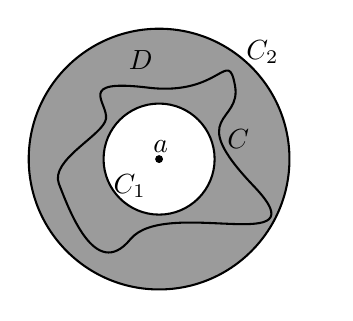
\begin{tikzpicture}[x=0.4pt,y=0.4pt,yscale=-1,xscale=1]
%uncomment if require:
\path (0,240.79999542236328);
%set diagram left start at 0, and has height of 240.79999542236328

%Shape: Circle [id:dp6258198346024846] 
\draw  [fill={rgb, 255:red, 155; green, 155; blue, 155 }  ,fill opacity=1 ] (0.77,120.35) .. controls (0.77,55.3) and (53.5,2.57) .. (118.55,2.57) .. controls (183.6,2.57) and (236.32,55.3) .. (236.32,120.35) .. controls (236.32,185.4) and (183.6,238.12) .. (118.55,238.12) .. controls (53.5,238.12) and (0.77,185.4) .. (0.77,120.35) -- cycle ;
%Shape: Circle [id:dp07560041299187703] 
\draw  [fill={rgb, 255:red, 255; green, 255; blue, 255 }  ,fill opacity=1 ] (68.39,120.35) .. controls (68.39,92.65) and (90.85,70.19) .. (118.55,70.19) .. controls (146.25,70.19) and (168.71,92.65) .. (168.71,120.35) .. controls (168.71,148.05) and (146.25,170.51) .. (118.55,170.51) .. controls (90.85,170.51) and (68.39,148.05) .. (68.39,120.35) -- cycle ;
%Shape: Circle [id:dp4185264747557642] 
\draw  [fill={rgb, 255:red, 0; green, 0; blue, 0 }  ,fill opacity=1 ] (116,120.35) .. controls (116,118.94) and (117.14,117.8) .. (118.55,117.8) .. controls (119.96,117.8) and (121.1,118.94) .. (121.1,120.35) .. controls (121.1,121.76) and (119.96,122.9) .. (118.55,122.9) .. controls (117.14,122.9) and (116,121.76) .. (116,120.35) -- cycle ;
%Shape: Polygon Curved [id:ds19792072871438626] 
\draw   (108.6,55.8) .. controls (174.6,63.8) and (180.6,18.8) .. (187.1,53.8) .. controls (193.6,88.8) and (141,78.8) .. (204.1,144.8) .. controls (267.2,210.8) and (124.6,153.8) .. (92.6,192.8) .. controls (60.6,231.8) and (36.72,164.55) .. (28.1,142.8) .. controls (19.47,121.05) and (68.77,98.46) .. (70.6,83.8) .. controls (72.43,69.14) and (42.6,47.8) .. (108.6,55.8) -- cycle ;

% Text Node
\draw (120,108.8) node    {$a$};
% Text Node
\draw (102,30.8) node    {$D$};
% Text Node
\draw (92,144.8) node    {$C_{1}$};
% Text Node
\draw (212,23.8) node    {$C_{2}$};
% Text Node
\draw (190,101.8) node    {$C$};

\end{tikzpicture}

\end{wrapfigure}
複素関数$f(z)$が点$a$を孤立特異点に持つとする。
また、点$a$を中心とする円$C_1, C_2$
($C_1$の中に$a$以外の特異点があっても良く、
$C_2$は$C_1$の外側にあるとする)
によって囲まれる領域を$D$とする。
$C_1, C_2$上、領域$D$のいずれにも特異点がないとき、
領域$D$内の任意の$z$に対し、
$D$内にあって$C_1$を囲むような単純閉曲線$C$を使って
\begin{subequations}
\begin{align}
    f(z)
    &= \sum_{n=-\infty}^{\infty}
        c_n (z-a)^n
\label{Laurent series expansion}
\\
    c_n
    &:= \dfrac{1}{2 \pi i}
    \oint_C dz_0 \dfrac{f(z_0)}{(z_0 - a)^{n+1}}
\end{align}
\end{subequations}
が成り立つ。
これを$f(z)$の$a$周りでのLaurent級数展開という。
特に(\ref{Laurent series expansion})の右辺のうち
$c_{-n}\ (n > 0)$が現れる項を特異部(singular part、主要部、principal part)、
$c_{n}\ (n \ge 0)$が現れる項を正則部(regular part、analytic part)という。

\subsubsection{極(pole)、真性特異点(essential singularity)、零点(zero)}

極とは、以下に定める孤立特異点の一種である。
$f(z)$が$a$を$m\ (>0)$位の極($m$-th order pole)
に持つとは、
$f(z)$のLaurent級数展開が$c_{-m} \neq 0$かつ
$n>m$に対し$c_{-n}=0$を満たすことを言う。
特に$1$位の極を単純極(simple pole)、
$2$位の極を二重極(double pole)、
$3$位ならtriple pole、などともいう。

Laurent展開の特異部が有限次で切れず
負べきの項が無限個現れる場合、
$a$を真性特異点(essential singularity)という。

$f(z)$が$a$を$m$位の零点($m$-th order zero)
に持つとは、
$f(z)$のTaylor級数展開が$c_{m} \neq 0$かつ
$n>m>0$に対し$c_{n}=0$を満たすことを言う。
零点は孤立する。

\subsubsection{留数定理(Residue theorem)}

Laurent級数展開
\begin{align}
    f(z)
    &= \sum_{n=-\infty}^{\infty}
        c_n (z-a)^n
\end{align}
において、
$\Res{f(z)dz, a} := c_{-1}$を
$f(z)$の点$z=a$における留数(Residue)という。
ただし本来これはRiemann球面$\mathbb{C}P^1$上の
微分形式に対し定義されるものだと示すため、
単に$f(z)$ではなく$f(z)dz$と書いた。
特に、
$f(z)$が$a$を$m$位の極
に持つときは
\begin{align}
    \Res{f(z)dz, a}
    =
    \lim_{z \to a}
    \dfrac{1}{(m-1)!}
    \dfrac{d^{m-1}}{dz^{m-1}}
    \bigg[
        (z-a)^m f(z)
    \bigg]
\end{align}
が成り立つ。
$f(z)$が単純閉曲線$C$内で
$n$個の孤立特異点$a_1,\dots,a_n$を除き正則であるとき
\begin{align}
    \oint_C dz\ f(z)
    =
    2 \pi i \sum_{k=1}^n
    \Res{f(z)dz, a_k}
\end{align}
が成り立つ。

\subsubsection{Morera's theorem(モレラの定理)}

以下の意味で、Cauchyの積分定理の逆が成り立つ:
単連結領域$D$で$f(z)$が連続で、
\begin{align}
    \oint_C dz\ f(z) = 0
\end{align}
が$D$内の任意の閉曲線$C$に対し成り立つとする。
このとき$f(z)$は$D$上で正則である。

\subsection{特殊関数}

\subsubsection{$\Gamma$関数}

$\Gamma$関数は$\Re z > 0$の複素数$z$に対し
\begin{align}
    \Gamma(z)
    := \int_0^\infty dt\ t^{z-1} e^{-t}
\end{align}
により定義され、
その性質
$\Gamma(1) = 1, \Gamma(z+1) = z\Gamma(z)$
から階乗
\begin{align}
    \Gamma(n+1) &= n!
    \quad
    (n \in \mathbb{N}_{\ge0})
\end{align}
の複素数への一般化を与える。

重要な応用として、
Gaussian integral(ガウス積分)
\begin{align}
    I :=
    \Gamma\left(\dfrac{1}{2}\right)
    =
    \int_{0}^{\infty} dt\ t^{-1/2}e^{-t}
    =
    2
    \int_{0}^{\infty} dx\ e^{-x^2}
    =
    \int_{-\infty}^{\infty} dx\ e^{-x^2}
    > 0
    \quad(t=x^2)
\end{align}
を求める事を考えよう。
極座標に書き換えると
\begin{align}
    I^2 &=
    \int_{-\infty}^{\infty} dx
    \int_{-\infty}^{\infty} dy
    \ 
        e^{-(x^2 + y^2)}
=
    \int_0^{\infty} dr
    \int_0^{2\pi} r d\theta
    \ 
        e^{-r^2}
\notag\\&=
    2 \pi
    \int_0^{\infty} dr
    \ r 
        e^{-r^2}
=
    \pi
    \int_0^{\infty} dt\ e^{-t}
    \quad(t:=r^2,\ dt = 2 r dr)
\notag\\&=
    \pi\Gamma(1)
    = \pi
\end{align}
すなわち
$\Gamma\left(\dfrac{1}{2}\right)
= I = \sqrt{\pi}$
が求まる。

$\Gamma$関数の$\Re z < 0$への解析接続は
Euler's reflection formula
\begin{align}
    \Gamma(z) \Gamma(1-z)
    =
    \dfrac{\pi}{\sin(\pi z)}
\label{Euler's reflection formula}
\end{align}
で与えられ、
この公式からも
$\Gamma \left(\dfrac{1}{2}\right) = \sqrt{\pi}$
が確かめられる。
$\Gamma$関数は零点を持たないが
(\ref{Euler's reflection formula})からも分かるように
$n \in \mathbb{N}_{\ge0}$に対して
$x = - n$を$1$位の極に持ち、
その周りで
\begin{align}
    \Gamma(x)
    &=
    \dfrac{(-1)^n}{n!}
    \left(
        \dfrac{1}{x+n} - \gamma
        + \sum_{k=1}^n \dfrac{1}{k}
    \right)
    + \mathcal{O}(x+n)
\\
    \gamma
    &:=
    \lim_{n\to\infty}
    \left(
        \sum_{k=1}^n \dfrac{1}{k} 
        -
        \log n
    \right)
    \simeq 0.5772
\end{align}
と展開できる。
ただし$\gamma$は
Euler-Mascheroni constant(オイラー定数)である。


\section{量子力学の公式}

\subsection{交換関係・反交換関係の基本的な性質}

証明は読者の演習問題とする。
\begin{align}
    [\hat{A}, \hat{B}] &= - [\hat{B}, \hat{A}]
\\
    [\hat{A}, \hat{B}\hat{C}]
   &=
   \hat{B}[\hat{A}, \hat{C}]
+
    [\hat{A}, \hat{B}] \hat{C}
\label{A,BC to B(A,C) + (A,B)C}
\\
    [\hat{A}\hat{B}, \hat{C}]
   &=
   \hat{A}\{\hat{B}, \hat{C}\}
-
    \{\hat{A}, \hat{C}\} \hat{B}
\\
    \left(\hat{A}\hat{B}\right)^\dagger
    &=
    \hat{B}^\dagger\hat{A}^\dagger
\\
    [\hat{A}, \hat{B}]^\dagger
    &=
    [\hat{B}^\dagger, \hat{A}^\dagger]
\end{align}

Baker-Campbell-Hausdrff formulaは
\begin{align}
    e^{\hat{A}} e^{\hat{B}}
    &=
    \exp\left(
        \hat{A} + \hat{B}
        + \dfrac{1}{2}[\hat{A},\hat{B}]
        + \dfrac{1}{12}[\hat{A} - \hat{B},[\hat{A},\hat{B}]]
        + \cdots
    \right)
\label{BCH formula}
\end{align}
である。証明のためには
$e^{\hat{C}(t)}
= e^{t\hat{A}} e^{t\hat{B}}$
すなわち$\hat{C}(t) = \log (
    e^{t\hat{A}} e^{t\hat{B}}
)$とおき、
右辺のTaylor展開を計算した後
$t=1$とおけばよい。
特に交換関係が$c$-数
$[\hat{A},\hat{B}]=c$の場合は
交換子を$2$回以上取ると必ず消えるため
\begin{align}
    e^{\hat{A}} e^{\hat{A}}
    &=
    \exp\left(
        \hat{A} + \hat{B}
        + \dfrac{1}{2}c
    \right)
\label{simpler BCH formula}    
\end{align}
となる。

正準変数$[\hat{q}_i, \hat{p}_j] = i\hbar\delta_{ij}$
については興味深い事実が成り立つ。
$C_n := \dfrac{1}{i\hbar} [\hat{q}^n_i, \hat{p}_j]$について
\begin{align}
    C_{n+1}
    &=
    \dfrac{1}{i\hbar}
    [\hat{q}^{n+1}_i, \hat{p}_j]
    =
    \hat{q}_i 
    \dfrac{1}{i\hbar}
    [\hat{q}_i^n, \hat{p}_j]
    +
    \dfrac{1}{i\hbar}
    [\hat{q}_i, \hat{p}_j] \hat{q}_i^n
    =
    \hat{q}_i C_n
    +
    \delta_{ij} \hat{q}_i^n
\end{align}
なる漸化式が導けるが、
これは初期条件
$C_0  = 0, C_1 = \delta_{ij}$のもとで
容易に
\begin{align}
    C_{n+1} &= 
    \dfrac{1}{i\hbar}
    [\hat{q}^{n+1}_i, \hat{p}_j]
    = \delta_{ij} (n+1) \hat{q}^n
\label{differential by commutator}
\end{align}
と解け、多項式の微分と同じ振る舞いを与える。
全く同様に
$\dfrac{1}{i\hbar}
[\hat{q}_i, \hat{p}^{n+1}_j]
= \delta_{ij} (n+1) \hat{p}^n$
も示される。
一般にoperatorの関数$F$の定義
(\ref{function of operator})
はTaylor展開で与えられていたので、
\begin{align}
    \dfrac{1}{i\hbar}
    [F(\{ \hat{q} \},\{ \hat{p} \}), \hat{p}_i]
    &=
    \dfrac{
        \partial F(\{ \hat{q} \},\{ \hat{p} \})
    }{
        \partial q_i
    }
\\
    \dfrac{1}{i\hbar}
    [\hat{q}_j, F(\{ \hat{q} \},\{ \hat{p} \})]
    &=
    \dfrac{
        \partial F(\{ \hat{q} \},\{ \hat{p} \})
    }{
        \partial p_j
    }
\end{align}
なる公式が得られる。

任意のoperator $\hat{O}$に対し、
そのHeisenberg表示(Heisenberg描像、Heisenberg picture)を
\begin{align}
    \hat{O}(t)
    :=
    \exp\left(
        -\dfrac{\hat{H} t}{i\hbar}
    \right)
        \hat{O}
    \exp\left(
        +\dfrac{\hat{H} t}{i\hbar}
    \right)
\end{align}
のように定義する。
$\hat{H}$のSchr\"odinger描像とHeisenberg描像は
一致する。
また、もちろんSchr\"odinger描像で
$\hat{O}$自身が顕わに$t$に依存している場合も
Heisenberg描像は同様に定義できる。
Heisenberg描像のoperator
$F(\{ \hat{q} \},\{ \hat{p} \}, t)$と
$\hat{H}$との交換関係は
\begin{align}
    \dfrac{d}{d t}
    F(\{ \hat{q} \},\{ \hat{p} \}, t)
    =
    \dfrac{1}{i\hbar}
    [F(\{ \hat{q} \},\{ \hat{p} \}, t), \hat{H}]
    + \dfrac{\partial}{\partial t}
    F(\{ \hat{q} \},\{ \hat{p} \}, t)
    \label{Heisenberg e.o.m}
\end{align}
となり、Heisenberg equation of motionと呼ばれる。
これはPoisson括弧で書かれた正準方程式(\ref{Hamilton e.o.m. in Poisson bracket})
ないし任意の関数$F$の時間発展(\ref{time evolution in Poisson bracket})
と同一の構造であり、
量子化とは
$\{A, B\}_{ \mathrm{P} }$
を
$\dfrac{1}{i\hbar} [\hat{A}, \hat{B}]$
で置き換える操作である、という
Bohrの対応原理(correspondence principle)をある意味で正当化する。
もちろん\ref{subsubsec: CCR}節で述べたように、
一般にある古典力学系に対して
対応する量子力学系は一意に定まらないので
「古典系を量子化する」という操作はwell-definedではなく、
現代的にはむしろ
量子力学を十分低energyでmacroscopicな系に適用すると
古典力学を再現する、という理解が正しい。
